% README.tex
% Based on File acl2012.tex
%
% Contact: Maggie Li (cswjli@comp.polyu.edu.hk), Michael White (mwhite@ling.osu.edu)
%%
%% Based on the style files for ACL2008 by Joakim Nivre and Noah Smith
%% and that of ACL2010 by Jing-Shin Chang and Philipp Koehn


%\usepackage{setspace}
%\doublespacing

\documentclass[11pt]{article}
\usepackage{latexsym}
\usepackage{amsmath}
\usepackage{multirow}
\usepackage{url}
\usepackage{pgfplots}
\usepackage{cite}
\usepackage{framed}
\makeatother
\usepackage[hidelinks]{hyperref}
\DeclareMathOperator*{\argmax}{arg\,max}
\pgfplotsset{compat=1.14}

\begin{document}

\title{\vspace{-2.5cm}Optical Character Recognition through Convolutional Neural Networks}
\author{Jay Szeto\\ jsa143@sfu.ca \and Adrian Lim\\ aclim@sfu.ca}
\maketitle

\hrulefill

\section{Introduction}
    Optical Character Recognition (OCR) is the process of converting an image of text into a computer readable format. \cite{ocr_wiki_2017} It can be used in applications such as data entry, license plate recognition, and defeating CAPTCHA anti-bot systems.\cite{ocr_wiki_2017} One approach for OCR involves the segmentation of an image into characters before the classification of each character. Of the many different ways to classify an image, one of the more popular approaches involves the use of Convolutional Neural Networks (CNN). \cite{lecun_bottou_bengio_haffner_1998} This type of approach has grown more popular and complex in recent years which can be seen by the appearance of neural networks such as LeNet, ImageNet, and ResNet. \cite{lecun_bottou_bengio_haffner_1998, image_net_2012, he2016deep}
    
    Due to the popularity of deep learning in recent years, we have decided to focus on CNNs for this project. We construct multiple different CNNs using the TensorFlow library in order to classify digits, lower-case, and upper-case letters.\cite{tensorflow15-whitepaper} We have also attempted to implement a basic line and character segmentation algorithm to detect words in examples such as in text documents.
    
\section{Related Work}
TensorFlow uses an assortment of procedures to enable training.\cite{tensorflow15-whitepaper} This section will focus on highlighting existing concepts and mathematical applications that are core components in the tested neural network. Using these concepts, TensorFlow is able to facilitate the construction of different type of layers to construct neural networks.~\cite{aGuideToLayers17}

\iffalse
\textbf{TensorFlow provides a step-by-step tutorial on building a LeNet style CNN with dropout for classifying the MNIST data set.\cite{tensorflow15-whitepaper, lecun_bottou_bengio_haffner_1998} This provided a good starting point for applying a CNN to the Char74k data set.}
\fi
    
    
\subsection{Model Generation Function}
TensorFlow uses the softmax regression function to calculate loss when assigning weights.~\cite{mnist-for-ml-beginners17}  This model uses two steps:
\begin{enumerate}
  \item Collect a sum of evidence values from input belonging to a certain class.
  \item Convert that evidence into weights.
\end{enumerate}
Evidence is gathered by performing a weighted sum of the pixel intensities.  A negative weight for a pixel represents evidence that is against the image being in that class. Positive weights are treated as evidence in favor of labeling an image to said class.  Extra evidence, called bias, were also added.  These extra data allows the algorithm to affect the evidence with weights "more likely independent of the input".~\cite{mnist-for-ml-beginners17}  Evidence for a class i given an input x is:
\begin{equation}
    evidence_{i} = \sum W_{i,j}x_{j} + b_{i}
\end{equation}


where $W_{i}$ is the weight and $b_{i}$ is the bias for class $i$, $j$ being an index allowing the summation of the pixels of the input image $x$.  
Once these evidences are available, a normalization is required to create a valid probability distribution:
\begin{equation}
    softmax(x)_{i} = \frac{exp(x_{i})}{\sum exp(x_{j})}
\end{equation}


\iffalse
(Archived just in case)
\begin{equation}
    y = softmax(evidence)    
\end{equation}

\begin{equation}
    softmax(x) = normalise(exp(x))
\end{equation}

\begin{equation}
    softmax(x) = \frac{exp(x_{i})}{\sum_{j} exp(x_{j})}
\end{equation}
\fi


Exponentiation allows increases in evidence units to amplify our hypothesis of prediction probabilities multiplicatively. On the other hand, reduction in evidence amounts results in the hypothesis to reduce to a fraction of its former amount.~\cite{mnist-for-ml-beginners17}

\iffalse
(The "Implementing the Regression" in first MNIST tutorial is after. However, the ItR section contains implementation details, proper placement of such info may be required...)
\fi

\subsection{Error Minimization Algorithms}
Although a method for calculating probability via evidence is available, such a model requires a training process in order to output the desired outcome.  A model's effectiveness is measured by how minimal its error margin is.  A model's loss is measured through the cross-entropy function:
\begin{equation}
    H_{y'} = - \sum y'_{i} log(y_{i})
\end{equation}
Where $y$ is the predicted probability distribution, and $y'$ is the true distribution of probabilities.~\cite{mnist-for-ml-beginners17}

The minimization of the loss output function is the responsibility of the backpropagation algorithm.  By minimizing the loss function output, users can maximize the amount of confidence behind a model's prediction.  After evaluating the derivative of each weight, this algorithm can determine whether or not a weight must increase or decrease to minimize loss.~\cite{YannLecunBottouOrrMuller98}

Finally, a gradient descent algorithm will utilize the results of the backprogation algorithm to alter weights for determining a minimum cross entropy value.  Although TensorFlow provides a multitude of gradient descent variations, the tested neural network utilized TensorFlow's stochastic gradient descent algorithm.~\cite{aGuideToLayers17}




\subsection{Layers}
Neural networks consists of a different range of layer types.  Below are three different types that were used: convolutional, pooling, and fully connected layers.~\cite{aGuideToLayers17}
\begin{enumerate}
  \item \textbf{Convolutional Layer:} A layer that applies convolution, filters the input image with a ReLU activation function.  Each portion of the image will produce an individual value to the output map.~\cite{aGuideToLayers17}
  \item \textbf{Max Pooling Layer:} extracts the data from convolutional layers to reduce the dimensions of the received feature map.  Due to the max pooling algorithm, only the maximum values will persist after such downsampling.~\cite{aGuideToLayers17}
  \item \textbf{Fully Connected Layer:} Unlike the convolutional and pooling layers, a fully connected layer receives and outputs a map of a constant size.~\cite{aGuideToLayers17}
\end{enumerate}





\section{Approach}

    The Char74K's computer "EnglishFnt" data set was used for training and testing of the CNNs.  Such font data seemed to greatly reflect the type of characters we were trying to detect. This data set contained 62992 computer generated images of 62 classes of digits, lower-case, and upper-case letters. \cite{deCampos09} They consisted of 254 different fonts with 4 different styles; normal, bold, italic, and bold and italic. \cite{deCampos09} The images were additionally centered, padded, and were of a constant size of 128 x 128. \cite{deCampos09} Images from this data set can be seen in Figure \ref{fig:char74k_data}.
    
    To observe the effect of different parameters on the CNN, we constructed multiple networks using the TensorFlow library. In both CNNs, the Char74K data set was randomly split into a training set containing 90\% of the data, a validation set containing 5\% of the data, and a test set containing the remainder of the data. Validation and training accuracy was plotted to monitor for overfitting. these graphs can be seen in Figures \ref{fig:training_accuracy} and \ref{fig:validation_accuracy}.
    
    When training the network we used a batch size of 100. We also used 3 epochs of the training data. In the case of the 3 convolutional layer model, we stopped early as it appeared the results were not improving after multiple steps.
    
    \begin{figure}
    \centering
    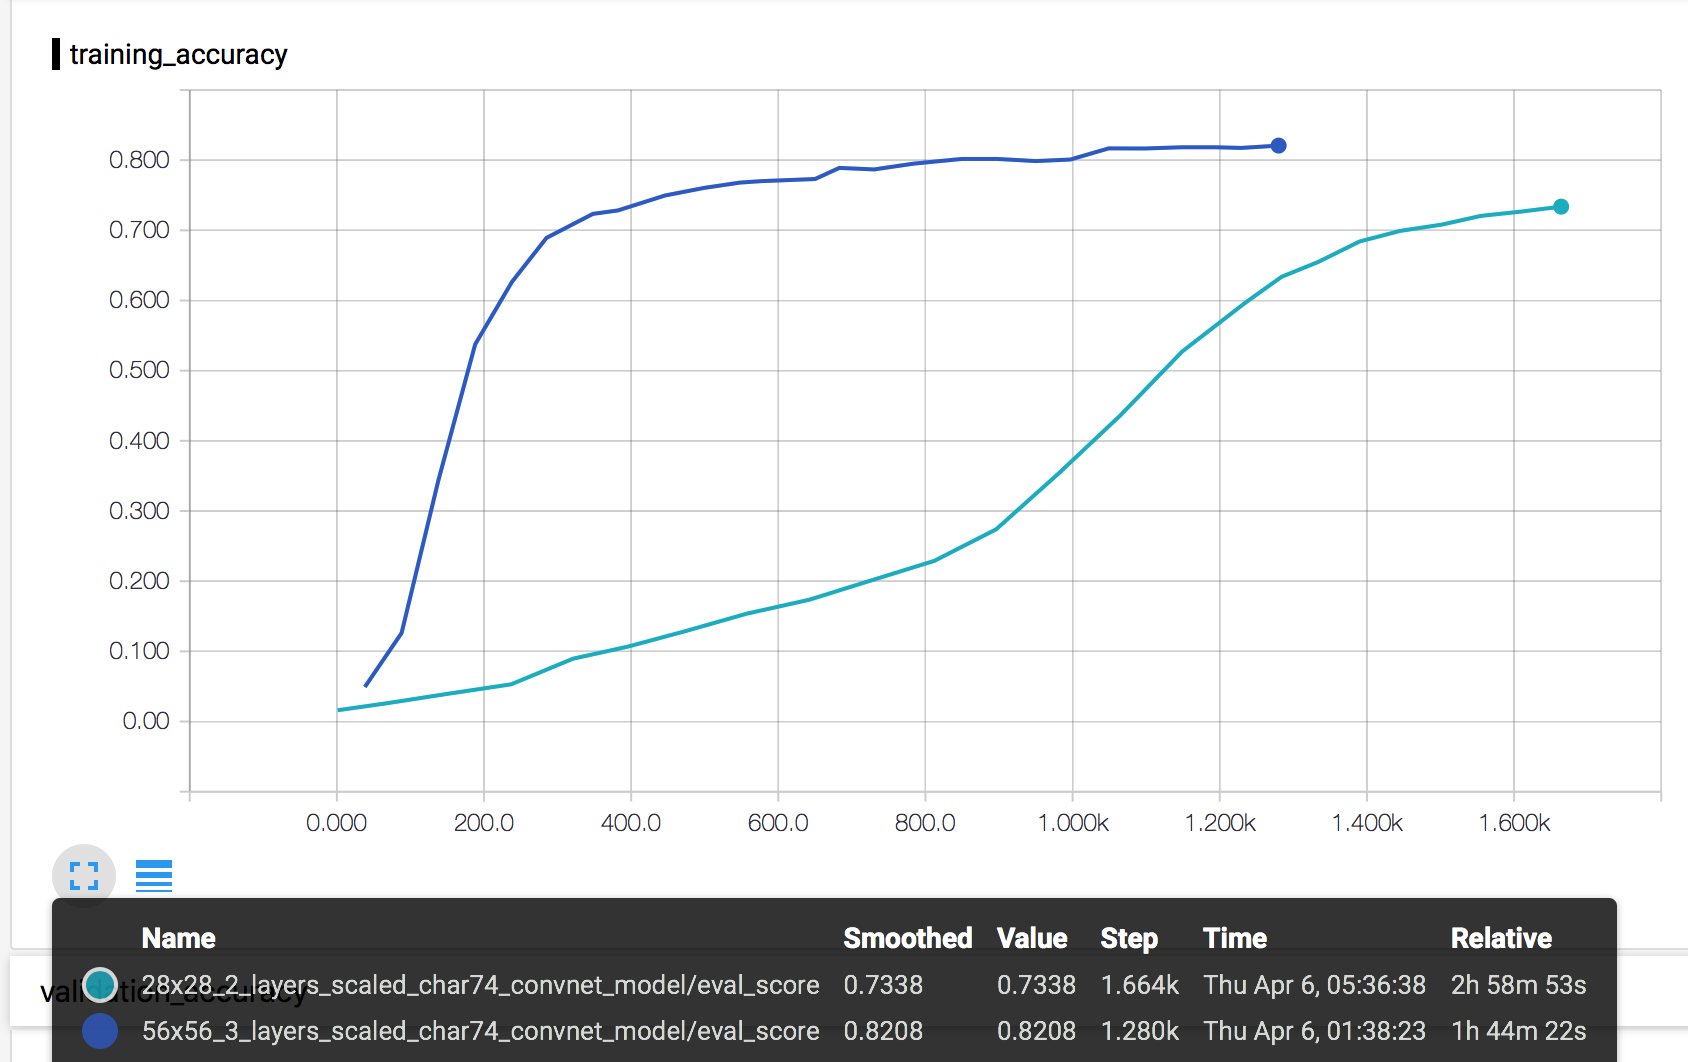
\includegraphics[scale=0.4]{training_accuracy.png}
    \caption{Training Accuracy}
    \label{fig:training_accuracy}
    \end{figure}

\begin{figure}
    \centering
    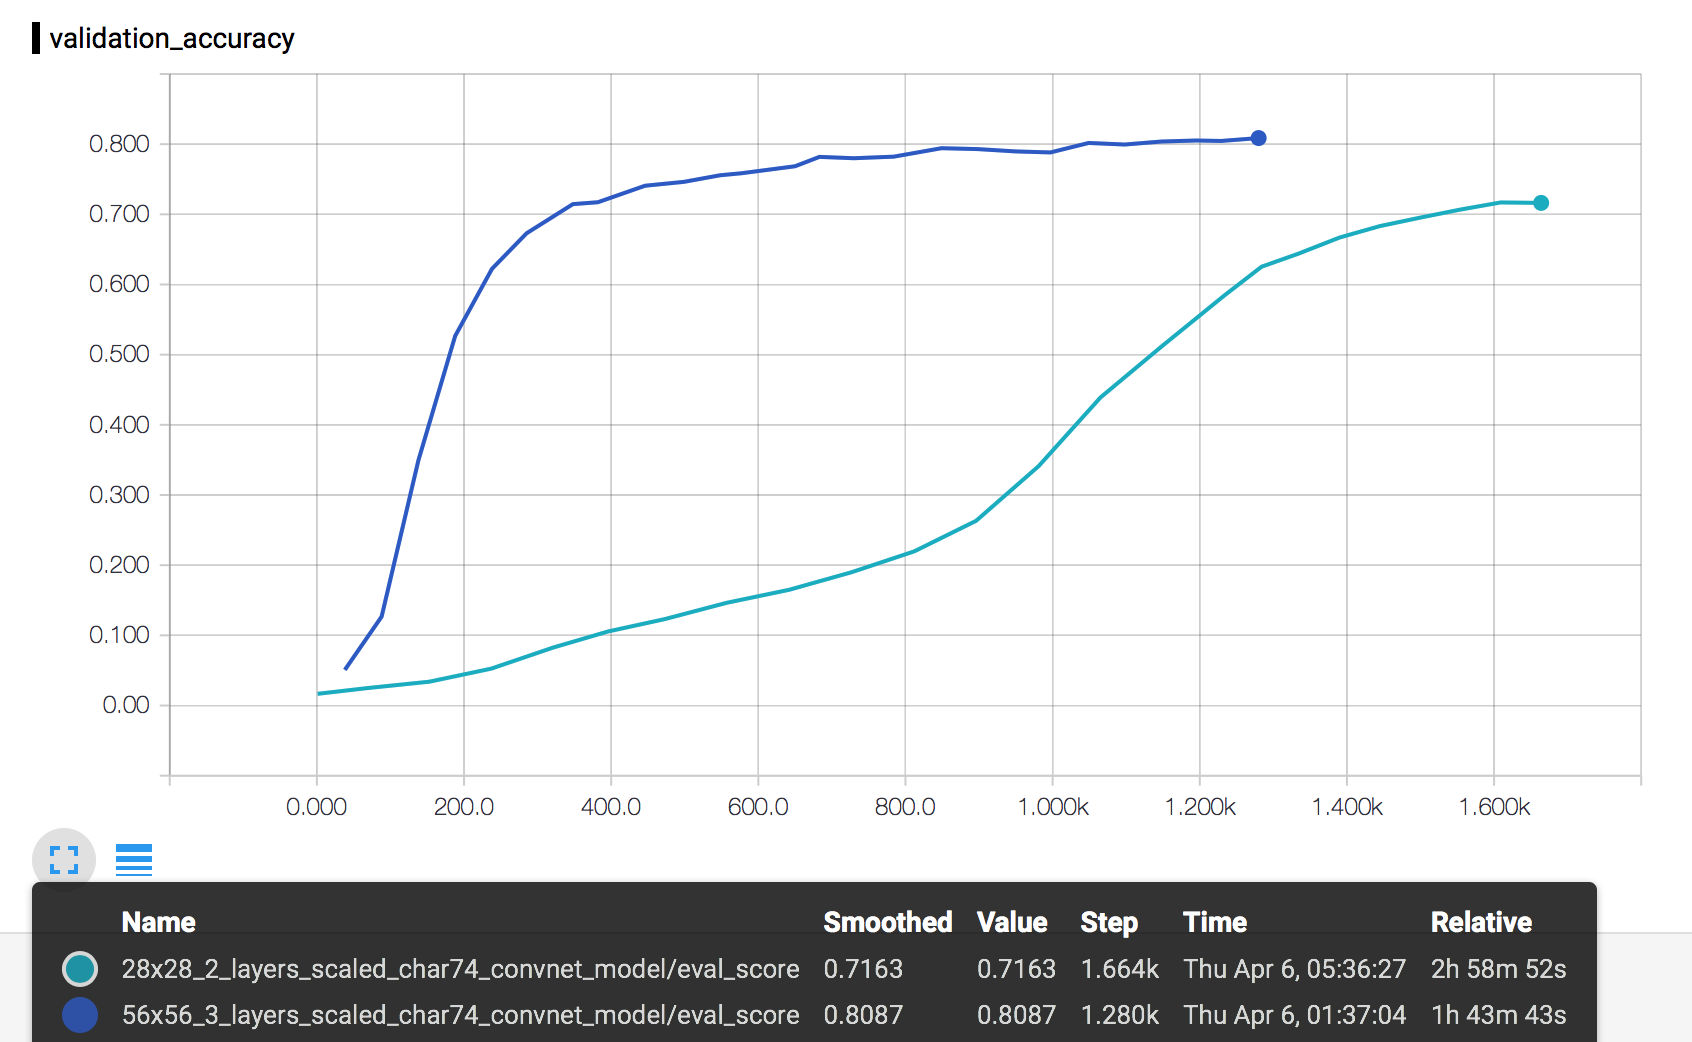
\includegraphics[scale=0.4]{validation_accuracy.png}
    \caption{Validation Accuracy}
    \label{fig:validation_accuracy}
\end{figure}
    
    \begin{figure}
        \centering
        
\includegraphics[scale=0.4]{training_data_sample.png}
        \caption{4 Images from the Char74k "EnglishFnt" Data Set}
        \label{fig:char74k_data}
    \end{figure}
    
    The first tested CNN was a modified version of the neural network in the MNIST TensorFlow tutorial. \cite{tensorflow15-whitepaper} The only modification that was made was that the final fully connected layer in the network was modified to output to 62 nodes rather than 10.  This is to reflect the 62 different character types in our training data. The image is first resized to 28 x 28. After, it is convolved with 32 filters with a kernel size of 5 x 5 in the first convolutional layer. In the first pooling layer, the image size is reduced by 2 by applying a pooling size of 2 x 2 with a stride of 2. In the second convolutional layer we apply 64 filters but keep the same kernel size as the first layer. This is followed by another pooling layer and 2 fully connected layers. To prevent overfitting we apply dropout to the first fully connected layer. The layer structure of the first CNN can be seen in Figure \ref{fig:model_1}.
    
    \begin{figure}
        \centering
        \begin{framed}
        CONV -\>> RELU -> POOL -> CONV ->RELU -> POOL -> FC -> RELU -> DROPOUT -> FC
        \end{framed}
        \caption{Model from TensorFlow Tutorial}
        \label{fig:model_1}
    \end{figure}
    
    Another CNN that was tested was an extended version of the previous network. In the newest neural network we doubled the size of the input image and added an additional convolutional layer and pooling layer. The added convolutional layer and pooling layer have the same parameters as the previous layer in the CNN.
    
    This CNN an be seen in Figure \ref{fig:model_2}.
    
    \begin{figure}
        \centering
        \begin{framed}
        CONV -\>> RELU -> POOL -> CONV ->RELU -> POOL -> CONV ->RELU -> POOL -> FC -> RELU -> DROPOUT -> FC
        \end{framed}
        \caption{Model with Additional Convolutional Layer and Pool Layer}
        \label{fig:model_2}
    \end{figure}
    
    In order to process images containing a set of characters, a way to normalize and segment characters in images was developed. This was accomplished using a basic algorithm that first segmented lines in the text. This was done by searching each row for white space. If a row consisted entirely of white space it was assumed that the end of the line was found. An example output from this line segmentation algorithm can be found in Figure \ref{fig:line_segmentation}. The characters were then isolated from each line by running the previous algorithm on each column. An example output from this character segmentation algorithm can be found in Figure \ref{fig:character_segmentation}. These characters were then scaled and padded appropriately and classified by the CNN.
    
    \begin{figure}
        \centering
        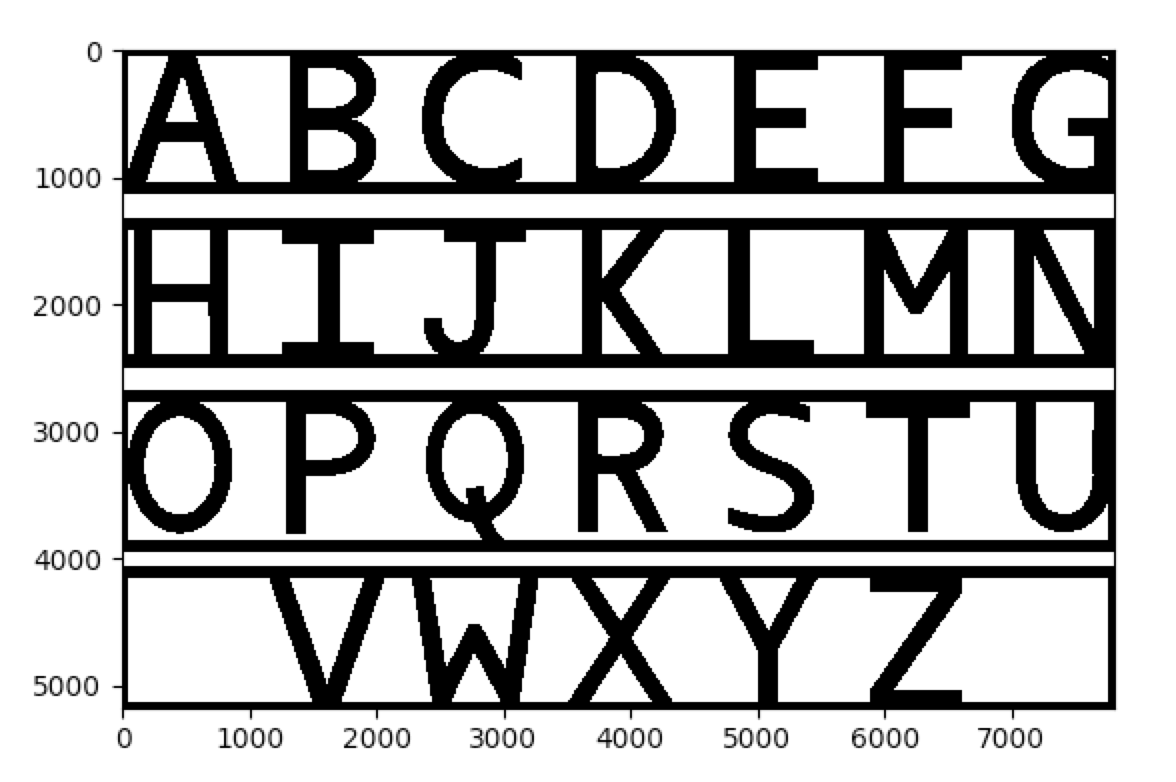
\includegraphics[scale=0.4]{line_segmentation_example.png}
        \caption{Line Detection and Segmentation}
        \label{fig:line_segmentation}
    \end{figure}   
    
    \begin{figure}
        \centering
        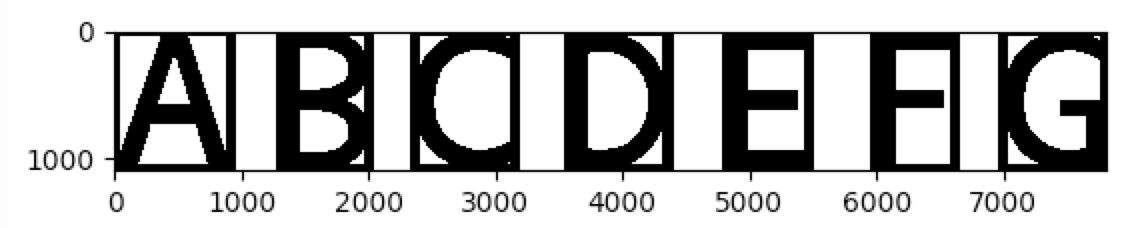
\includegraphics[scale=0.4]{character_segmentation_example.png}
        \caption{Character Detection and Segmentation}
        \label{fig:character_segmentation}
    \end{figure}

\section{Results}

The test set consists of 12600 images from the Chars74K data set. A number of images were programatically set aside for the test set but an error caused this set to become irretrievable. Due to the large amount of time required to retrain a new network with a new set, we decided to continue using the aforementioned 12600 random images from the complete set.

Using the TensorFlow MNIST tutorial modified example, we get a 74\% accuracy against our test set. A bar chart of the incorrectly predicted images can be seen in Figure \ref{fig:model_1_error}.

Our model with the added convolutional layer and pooling layer achieved an 81.8\% accuracy against our test set. A bar chart of the incorrectly predicted images can be seen in \ref{fig:model_2_error}.

\begin{figure}
    \centering
    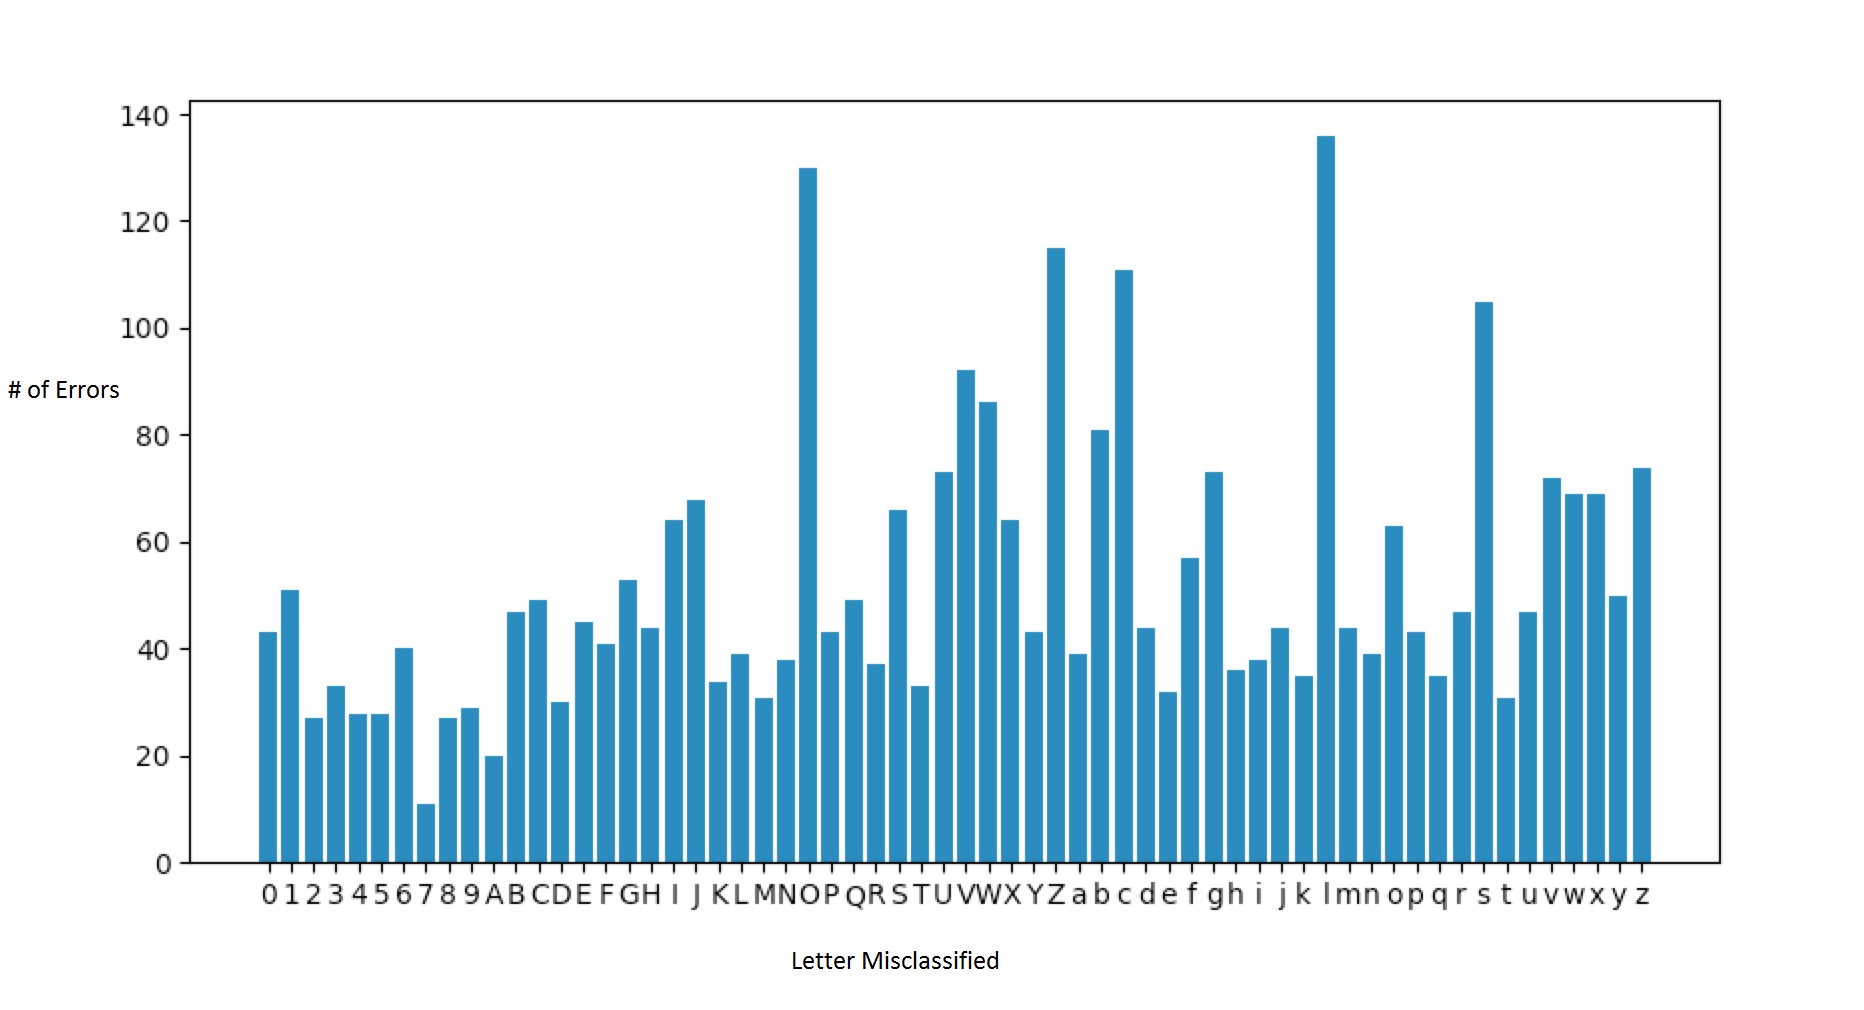
\includegraphics[scale=0.3]{model_1_errors-wlabels.png}
    \caption{Bar graph showing which sample images were misclassified in the TensorFlow example prediction}
    \label{fig:model_1_error}
\end{figure}

\begin{figure}
    \centering
    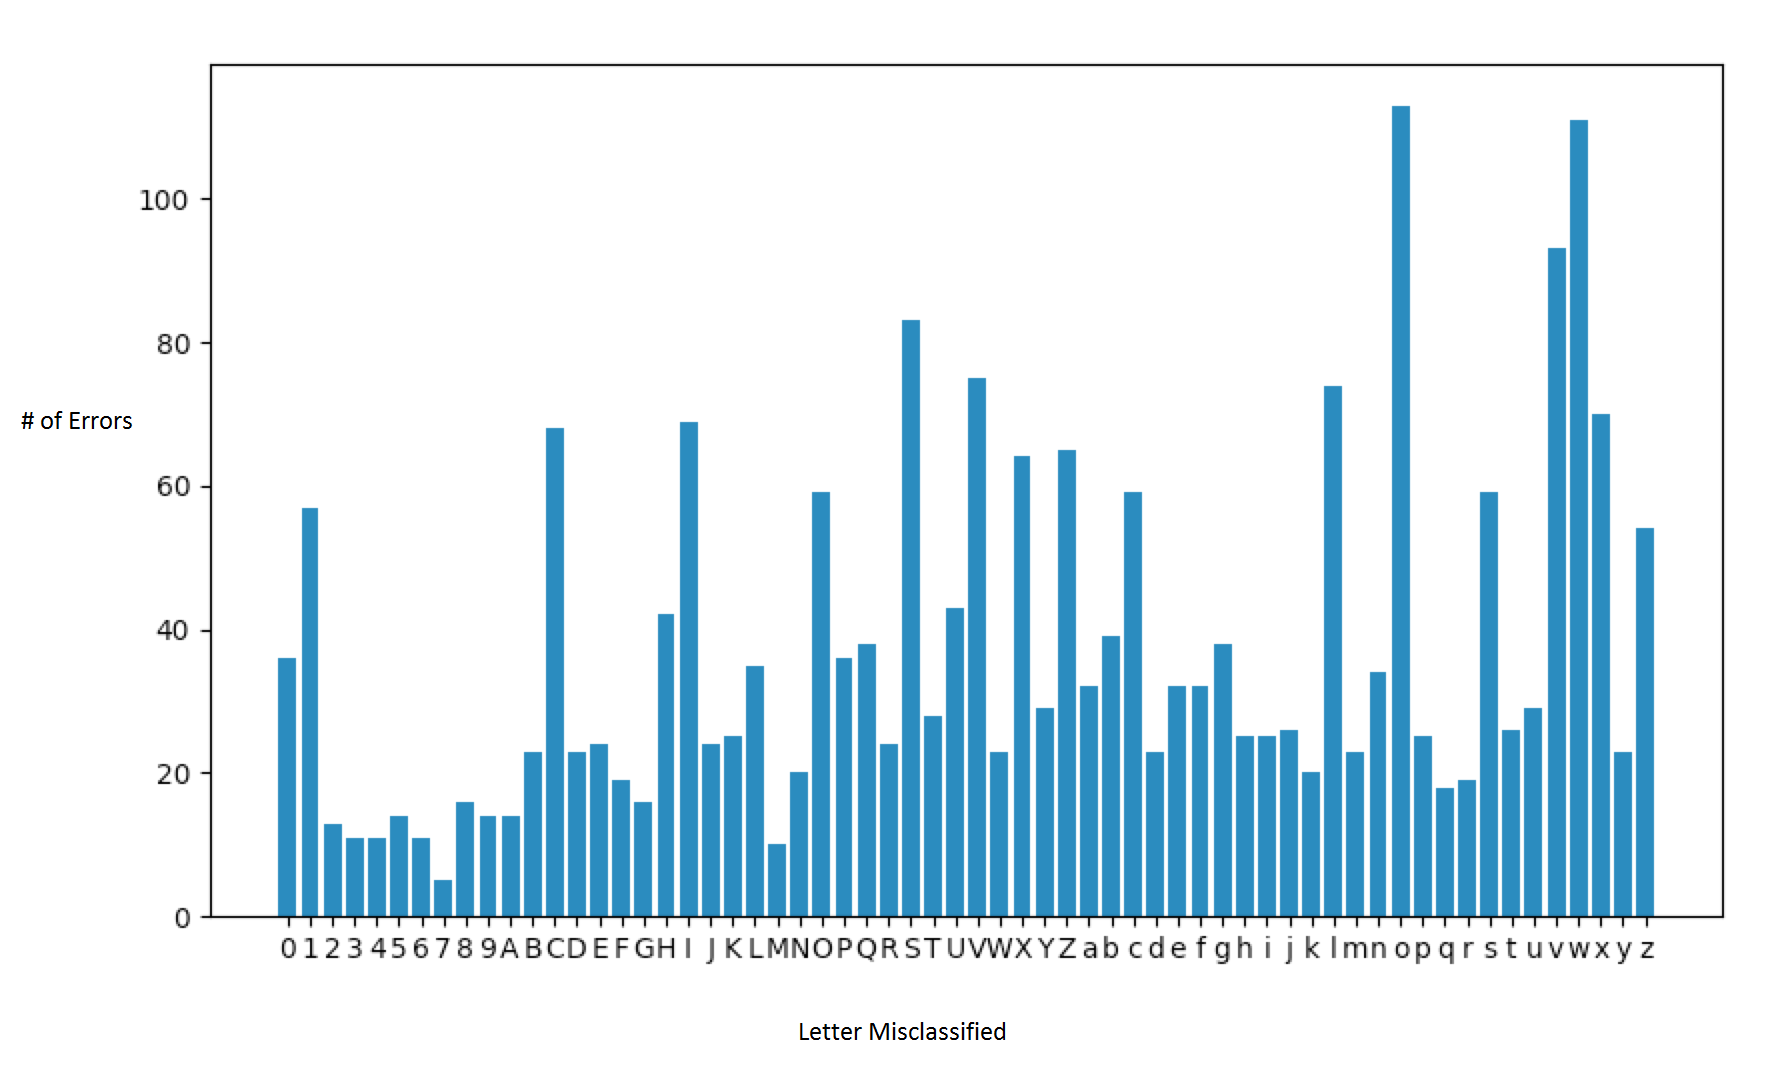
\includegraphics[scale=0.3]{model_2_errors-wlabels.png}
    \caption{Bar graph showing which sample images were misclassified in the 3 convolutional and pool layer model}
    \label{fig:model_2_error}
\end{figure}

The combined character segmentation algorithm and improved CNN was applied to the image in Figure \ref{fig:line_segmentation}. Every letter was predicted correctly except for the letter O which was misclassified as the number 0.

This was then applied to a more ambitious example, a sentence taken from Wikipedia. \cite{ocr_wiki_2017} Though the neural network was not trained with symbols other than the alphabet and numbers, and the segmentation algorithm was quite basic, the output from the program was still somewhat ledge-able. This is shown in Figure \ref{fig:sentence_ocr}.

\begin{figure}
    \centering
    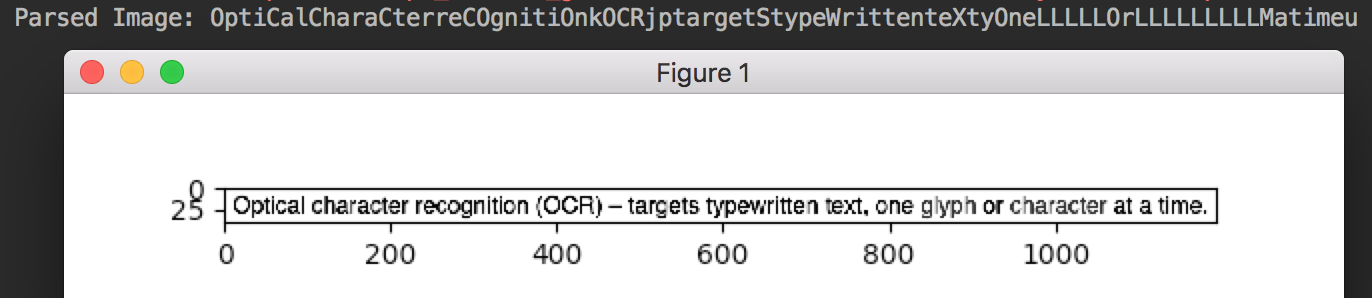
\includegraphics[scale=0.6]{sentence.png}
    \caption{OCR on a Sentence Image Taken from Wikipedia}
    \label{fig:sentence_ocr}
\end{figure}

\section{Discussion}

The results show that adding a convolutional layer and a pooling layer in the neural network increased the accuracy of the neural network by 7.8\%. However, this may be due to overfitting as we were unable to test our network against the actual test set. That being said, we monitored the networks for overfitting by plotting the accuracy in our training set and validation set which can be seen in Figures \ref{fig:training_accuracy} and \ref{fig:validation_accuracy}.  From observing these two graphs, the two networks do not appear to be overfitting, since the validation data is not decreasing.

Analysis of the misclassified images of the trained neural networks seems to show that the majority of errors occur in images that are extremely similar to other images, 0 and O or 1 and l, for example. Due to how the images were processed in the Char74k training set it makes sense that these images become almost indistinguishable from one another and would cause at least 1 of these characters to be misclassified more often. \ref{fig:0Oo} This suggests that it may be impossible to correctly distinguish certain characters from each other without additional information such as the letters surrounding the character of interest.

When attempting to classify segmented characters outside of our data set without normalizing the characters, the predictions would be poor. Once we normalized both the training data and the characters taken outside of the data set, these predictions became much better.

In order to apply this OCR solution to text documents, a better segmentation algorithm will need to be implemented.

\begin{figure}
    \centering
    
\includegraphics[scale=0.4]{0Oo.png}
    \caption{From left to right: 0, O, o from the Char74K training set}
    \label{fig:0Oo}
\end{figure}

The results of the character segmentation shows that there is much room for improvement. However, a very basic character segmentation algorithm was written solely to apply our CNN on a more practical and interesting example.


\section{Future Work}

There are multiple areas that could be conducted to improve accuracy in our program. First, the data set that was used in the experiment did not contain punctuation which is critical for processing a text document. This could be addressed by adding these images to our data set and increasing the number of classes in our CNN. Another way we could improve our program for OCR would be to implement a better character segmentation program which could account and report spaces between words. Finally the character segmentation algorithm currently does not account for images in text, a pattern matching algorithm could be used to obtain solely the part of the image containing text.

\section{Conclusion}
Our results show that the CNN reported decent results if the input data was normalized correctly. In order to create an end-to-end OCR solution a better segmentation algorithm would need to be implemented. The results also show that it is difficult to classify the differences between similar characters such as O and 0 especially if the data is normalized in a similar way as in our data set. Although adding additional layers may increase over fitting as described in the ResNet paper, in our case it did not negatively impact our results and instead improved them. \cite{he2016deep}


\iffalse
Option: talk about Matt's ramblings on "Number plate recognition with TensorFlow" algorithm
and compare it to ours. (His approach, more training images/test data that are also indepth)
sliding window implementation to locate text region.
- pros: can detect meme text better
- cons: dataset for training images of text on pictures (meme format) not available
    - his algorithm only shows him detecting one plate (or line of text in the case of memes)
    - datasets are extensive example had ~3 GB of background images) tar file 36 GB
        - extracting tar file gets 108,634 images \url = {https://github.com/matthewearl/deep-anpr/blob/master/README.md}
    - his approach uses a specific font (good if meme follows consistent font, which isn't always the case since meme's are not regulated)


-------------------
Below are some brainstormed ideas for future work (Not exhaustive.  Section open to other ideas): 

- what can be improved 
    - e.g. character segmentation, 
    - ways to deal with noise, 
    - increasing number of layers...
    - etc
    
- what could we have done (if we had more time or resources...
    - e.g. specific details of how to char segmentation
    - noise dealing details
    - using specialized training images for specific
        reading situations
    
- how can we extend this further? What challenges will one might have to face?
    - e.g. algorithm to read documents...
    - text on meme reader
    - text on textbook reader (digital source)
    - text on a piece of paper (can easier be more noise)
        - but as similar in accuracy when reading from digital source, (suppose we read from high definition image of real textbook page to convert into digital source?
            - more issues if we make such a product since currently we assume text is parallel/horizontal
\fi

\iffalse
*Note: Future improvement, research showed that performing OCR (using...) is more effective in analyzing characters at the word level
http://yann.lecun.com/exdb/publis/pdf/lecun-95b.pdf

*Note: lowercase letters same "size" as uppercase in dataset
http://yann.lecun.com/exdb/publis/pdf/lecun-01a.pdf



\section{Note to Self/Sources/References?(use bibliography instead of this section)}
Certain Tutorials were provided by TensorFlow regarding how to create our own MNIST Convolutional Neural Networks
\begin{verbatim}
https://www.tensorflow.org/get_started/mnist/mechanics
https://www.tensorflow.org/tutorials/layers
\end{verbatim}

\fi



\clearpage
\bibliography{project}
\bibliographystyle{ieeetr}

\end{document}
